% Add this subsection to the ablation study section

\subsubsection{Semantic Boundaries: A Case Study at the Phase Transition}

The phase transition at $\theta \approx 0.875$ reveals more than statistical network fragmentation—it exposes \emph{semantic boundaries} between distinct conversational contexts. Figure~\ref{fig:niece_emergence} illustrates a compelling example: conversations with the author's 13-year-old niece that remain isolated at threshold 0.9 but connect to the giant component at 0.875.

\begin{figure}[h]
\centering
\begin{subfigure}{0.48\textwidth}
    \centering
    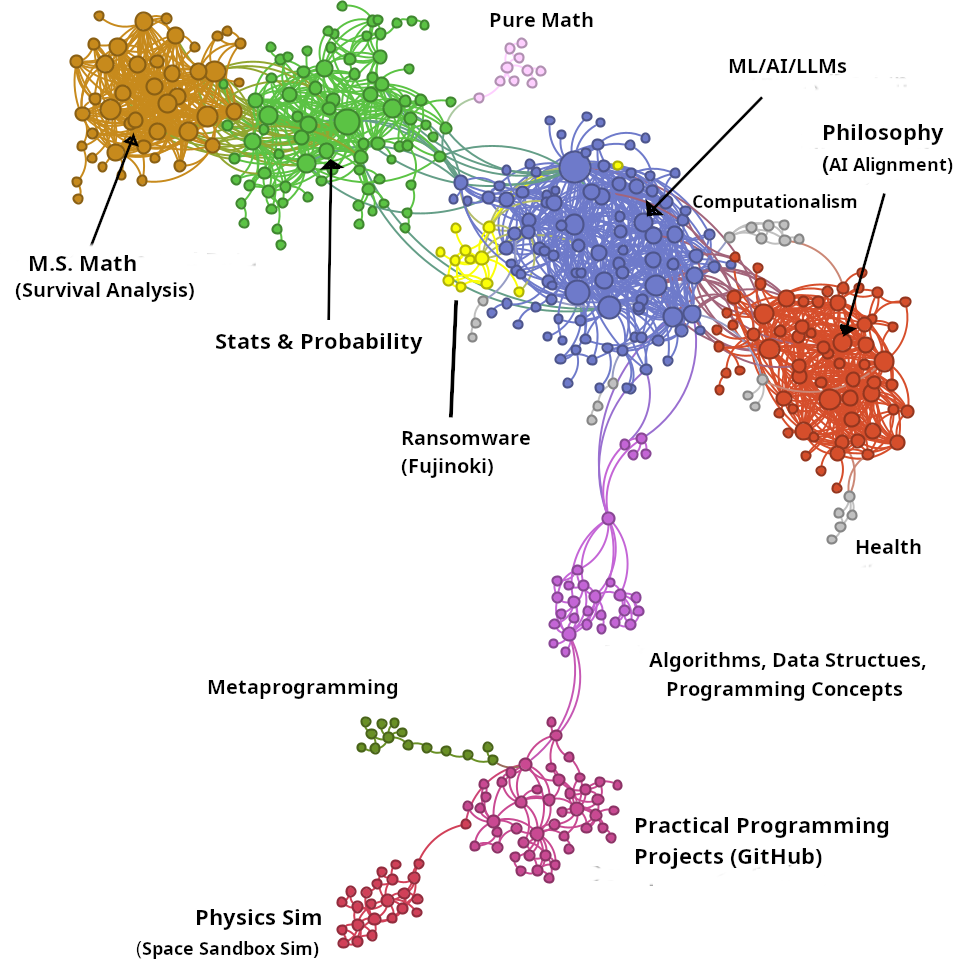
\includegraphics[width=\textwidth]{./images/cluster-vis-topics-better.png}
    \caption{Threshold 0.9: Niece conversations isolated}
    \label{fig:network_09}
\end{subfigure}
\hfill
\begin{subfigure}{0.48\textwidth}
    \centering
    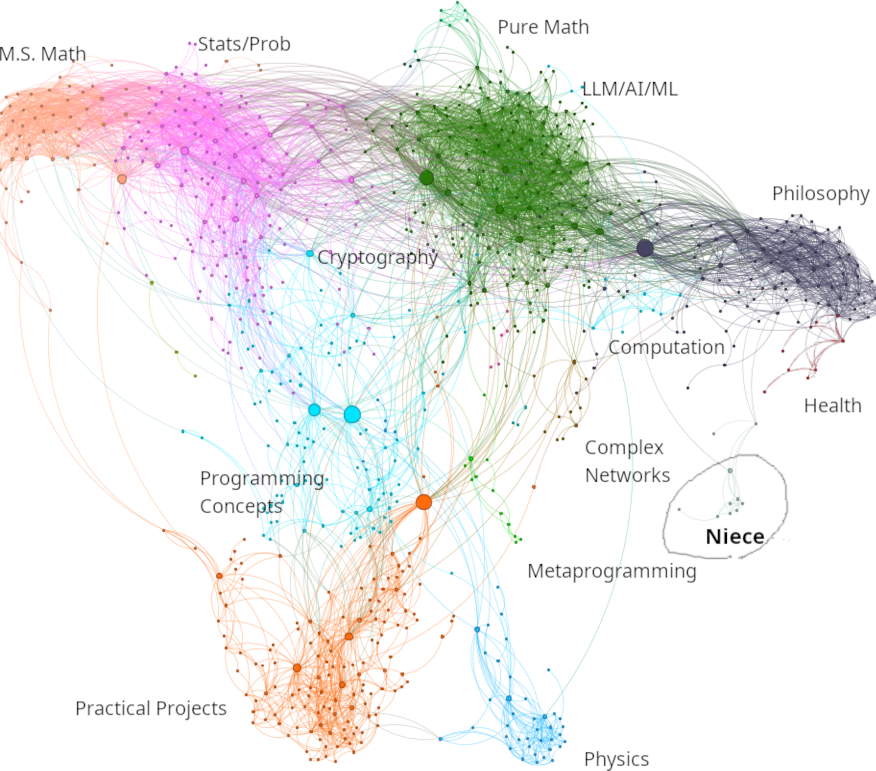
\includegraphics[width=\textwidth]{./images/0.875-wild-better.png}
    \caption{Threshold 0.875: Niece community emerges (pink, bottom)}
    \label{fig:network_0875}
\end{subfigure}
\caption{Semantic boundary crossing at the phase transition. At $\theta=0.9$ (left), the niece's conversations remain isolated due to distinct vocabulary and topics. At $\theta=0.875$ (right), they connect through philosophical bridge conversations, revealing a 12.5\% semantic similarity gap between conversational contexts.}
\label{fig:niece_emergence}
\end{figure}

This emergence demonstrates that the 2.5\% difference in similarity threshold (from 0.9 to 0.875) captures a fundamental semantic distance between:
\begin{itemize}
    \item \textbf{Primary knowledge network}: Technical discussions with consistent vocabulary, formal register, and domain-specific terminology
    \item \textbf{Peripheral conversational context}: Artistic topics, informal language, age-appropriate explanations, creative storytelling
\end{itemize}

The connection occurs through \emph{philosophical bridge} conversations where abstract concepts (consciousness, creativity, ethics) provide semantic overlap despite stylistic differences. This validates our choice of $\theta=0.9$ for analytical clarity—it preserves distinct cognitive contexts while the lower threshold reveals their latent connections.

\subsubsection{Implications for Threshold Selection}

This case study illustrates why threshold selection represents more than a technical parameter—it functions as a \emph{semantic filter} that determines which cognitive contexts merge or remain separate:

\begin{itemize}
    \item \textbf{$\theta = 0.9$}: \emph{Analytical threshold}—preserves context boundaries, suitable for studying focused knowledge domains
    \item \textbf{$\theta = 0.875$}: \emph{Discovery threshold}—reveals cross-context connections, suitable for exploring cognitive bridges
    \item \textbf{$\theta = 0.85$}: \emph{Integration threshold}—merges most contexts, suitable for holistic conversation analysis
\end{itemize}

The niece community's emergence precisely at the phase transition suggests this critical threshold approximates the natural semantic distance between distinct discourse domains within a single user's conversation history. This finding has implications for:

\begin{enumerate}
    \item \textbf{Personalization systems}: Different thresholds could surface contextually appropriate conversations
    \item \textbf{Privacy considerations}: Semantic boundaries might naturally separate professional from personal conversations
    \item \textbf{Cognitive modeling}: Phase transitions in conversation networks may reflect fundamental limits of semantic coherence
\end{enumerate}